\documentclass[mathserif]{beamer}
\usepackage[utf8]{inputenc}

% packages
\usepackage{physics}
\usepackage{amsfonts, amsmath, amssymb, amsthm}
\usepackage{systeme}
\usepackage[none]{hyphenat}
\usepackage{fancyhdr}
\usepackage{graphicx}
\graphicspath{{./images/}}
\usepackage{float}
\usepackage{siunitx}
\usepackage{esint}
\usepackage{cancel}
\usepackage{mathtools}

% colors
\usepackage{xcolor}
\definecolor{p}{HTML}{FFDDDD}
\definecolor{g}{HTML}{D9FFDF}
\definecolor{y}{HTML}{FFFFCF}
\definecolor{b}{HTML}{D9FFFF}
\definecolor{o}{HTML}{FADECB}
%\definecolor{}{HTML}{}

% \highlight[<color>]{<stuff>}
\newcommand{\highlight}[2][p]{\mathchoice%
  {\colorbox{#1}{$\displaystyle#2$}}%
  {\colorbox{#1}{$\textstyle#2$}}%
  {\colorbox{#1}{$\scriptstyle#2$}}%
  {\colorbox{#1}{$\scriptscriptstyle#2$}}}%

% paragraph indentation/spacing
\setlength{\parindent}{0cm}
\setlength{\parskip}{5pt}
\renewcommand{\baselinestretch}{1.25}

\newcommand{\br}[1]{\left(#1\right)}
\newcommand{\sbr}[1]{\left[#1\right]}
\newcommand{\cbr}[1]{\left\{#1\right\}}

\usetheme{Madrid}
\usecolortheme{default}

\renewcommand{\qedsymbol}{\textcolor{black}{\openbox}}

%------------------------------------------------------------
%This block of code defines the information to appear in the title page
\title[Another proof for the infinitude of primes] %optional
{Another proof for the infinitude of primes}

\subtitle{using elementary methods}

\author[Sai Sivakumar] % (optional)
{Sai Sivakumar}

\AtBeginSection[]{
  \begin{frame}
  \vfill
  \centering
  \begin{beamercolorbox}[sep=8pt,center,shadow=true,rounded=true]{title}
    \usebeamerfont{title}\insertsectionhead\par%
  \end{beamercolorbox}
  \vfill
  \end{frame}
}

\begin{document}

%The next statement creates the title page.
\frame{\titlepage}

%This block of code is for the table of contents after the title page
\begin{frame}
\frametitle{outline}
\tableofcontents
\end{frame}

\begin{frame}
  \frametitle{statement}
  \begin{theorem}
    There are infinitely many prime numbers.
  \end{theorem}
  \textit{Proof.} (variation of Euler's?)
  \[\vdots\]
\end{frame}

\section{setting up}

\begin{frame}
  \frametitle{the number of primes less than $x$}
  Let $\pi(x) \coloneqq \abs{\mathbb{P}_{\leq x}}$, where $\mathbb{P}_{\leq x} = \cbr{p\leq x\mid p \in\mathbb{P}}$, be the number of primes which are less than or equal to the real number $x$.

  Number the primes in ascending order so that we can write \[\mathbb{P} = \cbr{p_1,p_2,p_3,\dots}\text{ and }\mathbb{P}_{\leq x} = \cbr{p_1,p_2,\dots,p_{\pi(x)}},\] where $p_1 < p_2 < \cdots < p_{\pi(x)} < \cdots$.

  We wish to show that $\pi(x)$ is unbounded.
\end{frame}

\begin{frame}
  \frametitle{comparing areas}
  Let $n = \lfloor x \rfloor \leq x < n+1$ and consider the two integrals \[\int_1^x \frac{1}{t}\dd{t} \text{ and } \int_1^{n+1} \frac{1}{\lfloor t \rfloor}\dd{t}.\]

  The first integral is equal to $\log(x)$ (by definition) and the second one is equal to \[\sum_{i=1}^n\frac{1}{i} = 1 + \frac{1}{2} + \cdots + \frac{1}{n-1} + \frac{1}{n}.\]
\end{frame}

\begin{frame}
  \frametitle{new frame}

  \begin{columns}
    \frametitle{comparing areas}
    \column{0.5\textwidth}
    Furthermore, note that \[\log(x)\leq \sum_{i=1}^n\frac{1}{i}.\] This is most apparent with the image from the textbook.
    
    \column{0.5\textwidth}
    \begin{figure}[h]
      \centering
      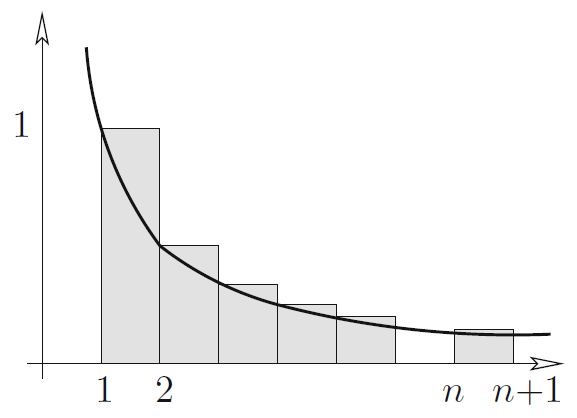
\includegraphics[scale=0.4]{areas}
    \end{figure}
  \end{columns}
\end{frame}

\section{getting leverage}

\begin{frame}
  \frametitle{new summation}
  Now consider the infinite sum \[\sum \frac{1}{m},\] where we sum over all $m\in \mathbb{N}$ which may have only prime divisors which are less than or equal to $x$. In other words, only primes $p\in\mathbb{P}_{\leq x}$ could divide each $m$.
\end{frame}

\begin{frame}
  \frametitle{this sum is larger?}
  We will show that this new sum, $\sum m^{-1}$, is larger than $\sum_{i=1}^n i^{-1}$ and hence larger than $\log(x)$.

  Observe that each of the terms in the sum $\sum_{i=1}^n i^{-1}$ are terms in this new sum, as every $i$ is less than $x$ and as a result all the prime divisors of each $i$ will be less than $x$. Then there will be infinitely many more extra nonzero terms in the sum, so we must have that this new sum exceeds $\log(x)$.
\end{frame}

\begin{frame}
  \frametitle{rewriting the new sum}
  We want to rewrite the sum \[\sum\frac{1}{m}\] in a more convenient manner.
  
  Recall the fundamental theorem of arithmetic says that every positive integer has a unique prime factorization (up to permutation of the prime factors).

  So each $m$ has a unique prime factorization given by some $\displaystyle{\prod_{p\in \mathbb{P}_{\leq x}} p^{k_p}}$.
\end{frame}

\begin{frame}
  \frametitle{cooler way to write the sum}
  We write \[\sum \frac{1}{m} = \prod_{p\in \mathbb{P}_{\leq x}}\br{\sum_{k=0}^{\infty} \frac{1}{p^k}},\] and to see how these are equal, observe how the full expansion can produce every term in the original sum: \[\br{\frac{1}{p_1}+\frac{1}{p_1^2}+\cdots}\br{\frac{1}{p_2}+\frac{1}{p_2^2}+\cdots}\cdots\br{\frac{1}{p_{\pi(x)}}+\frac{1}{p_{\pi(x)}^2}+\cdots}\]
\end{frame}

\begin{frame}
  \frametitle{algebra}
  Each sum in the product is a geometric series, so
  \[\log(x)\leq \prod_{p\in \mathbb{P}_{\leq x}}\br{\sum_{k=0}^{\infty} \frac{1}{p^k}} = \prod_{p\in \mathbb{P}_{\leq x}}\frac{1}{1-\frac{1}{p}} = \prod_{p\in \mathbb{P}_{\leq x}}\frac{p}{p-1} = \prod_{j = 1}^{\pi(x)}\frac{p_j}{p_j-1}.\] Furthermore, $p_j \geq j+1$, so we bound above each factor in the product: \[\frac{p_j}{p_j-1} = \frac{(p_j-1) + 1}{p_j-1} = 1 + \frac{1}{p_j-1} \leq 1+\frac{1}{j} = \frac{j+1}{j}\]
\end{frame}

\begin{frame}
  \frametitle{satisfying part}
  Finally see that \[\log(x) \leq \prod_{j = 1}^{\pi(x)}\frac{p_j}{p_j-1} \leq \prod_{j=1}^{\pi(x)}\frac{j+1}{j} = \pi(x)+1.\] So $\log(x)-1 \leq \pi(x)$, meaning we found a lower bound on the number of primes less than $x$. The lower bound, $\log(x)-1$, is unbounded, which implies $\pi(x)$ is unbounded as well and so we find there are infinitely many primes. \qed
\end{frame}

\end{document}